\documentclass[9pt,xcolor=table]{beamer}
\usepackage[latin1]{inputenc}
\usepackage[english]{babel}
% \usepackage{graphics}
\usepackage{graphicx}
\usepackage{hyperref}
\usepackage{units}
\usepackage{amsmath}
\usepackage{amsfonts}
\usepackage{amssymb}
\usepackage{color, colortbl}
\usepackage{amsmath}
%\usepackage{wrapfig}
\usepackage[normalem]{ulem}
%\usepackage{multirow}
\usepackage{verbments}
\usepackage{textcomp}

\usetheme{MPICBG}

\def\cpp{\texttt{C++}}
\def\cpu{\texttt{CPU}}
\def\gpu{\texttt{GPGPU}}
\def\Cuda{\texttt{CUDA}}


\AtBeginSection[] 
{
\begin{frame}<beamer>
\frametitle{Outline}
\vspace{-1.5\baselineskip}
\begin{columns}[t]
  \begin{column}{.1\textwidth}
    \hfill
  \end{column}
  \begin{column}{.75\textwidth}
    \huge
    \tableofcontents[currentsection,hideallsubsections]
  \end{column}
  \begin{column}{.1\textwidth}
    \hfill
  \end{column}
\end{columns}
\end{frame}
}
   
\begin{document}
     
\pgfdeclareimage[height=1.5cm]{MPIlogo}{img/CBGlogo}
\titlegraphic{ \pgfuseimage{MPIlogo}  }
 
 
\title[PerfVsDesign]{Performance Versus Design}
\subtitle{- Advanced Programming School 2014 -}
\author[P. Steinbach]{Peter Steinbach}
\date{}
\institute[MPI CBG]{Max Planck Institute of Molecular Cell Biology and Genetics\\Scientific Computing Facility}
\addtocounter{framenumber}{-1}
\renewcommand*\inserttotalframenumber{XX} 

 
{
\setbeamertemplate{footline}{} 
\maketitle
}

\begin{frame}[t]
\frametitle{Outline}
\vspace{-1.5\baselineskip}
\begin{columns}[t]
  \begin{column}{.1\textwidth}
    \hfill
  \end{column}
  \begin{column}{.75\textwidth}
    \huge
    \tableofcontents[hideallsubsections]
  \end{column}
  \begin{column}{.1\textwidth}
    \hfill
  \end{column}
\end{columns}
\end{frame}

\section[Why \cpp{}?]{Why \cpp{}?}
\begin{frame}
\frametitle{\insertsection{}}
\begin{block}{A Devil's Advocate Game}
  \Huge
  \begin{center}
    \alert{Why \cpp{}?}
  \end{center}
\end{block}
\end{frame}

\subsection{My view}
\begin{frame}[c]
\frametitle{\insertsectionhead{} : \insertsubsection}
\vspace{-1.\baselineskip}
\begin{columns}[t]
  \begin{column}{.48\textwidth}
    \begin{exampleblock}{Pros}
      \begin{itemize}
      \item
      \end{itemize}
    \end{exampleblock}
  \end{column}
  \begin{column}{.48\textwidth}
    \begin{alertblock}{Cons}
      \begin{itemize}
      \item
      \end{itemize}
    \end{alertblock}
  \end{column}
\end{columns}
\end{frame}

\part{Performance}
%\section[Performance]{Performance}
\section{A Definition}
\begin{frame}
\frametitle{\insertsectionhead{} : \insertpart{}
}
\vfill
\begin{block}{Etymology}
  \begin{description}
  \item[perform] from Middle English \textit{performen}, \textit{parfournen} (``to perform''), from Anglo-Norman \textit{performer}, \textit{parfourmer}, alteration of Old French \textit{parfornir}, \textit{parfurnir} (``to complete, accomplish, perform''), from \textit{par}- + \textit{fornir}, \textit{furnir} (``to accomplish, furnish''), \dots
  \item[ance] added to the stem of a verb to form a noun indicating a state or condition, such as result or capacity, associated with the verb.\\
    \begin{flushright}
      \small(\href{http://en.wiktionary.org/wiki/perform}{wiktionary})
    \end{flushright}

  \end{description}
\end{block}
\vfill
\begin{block}{Computer Performance}
  \begin{center}
    \dots is characterized by the amount of useful work accomplished by a computer system or computer network compared to the time and resources used.\\
  \end{center}
  \begin{flushright}
    \small(\href{http://en.wikipedia.org/wiki/Computer_performance}{wikipedia})
  \end{flushright}

  \end{block}
\vfill
\end{frame}

\section[Resources]{The resources available}
\subsection{Computers?}
\begin{frame}[c]
\frametitle{\insertsectionhead{}: \insertsubsection{}}
\begin{figure}[htb]
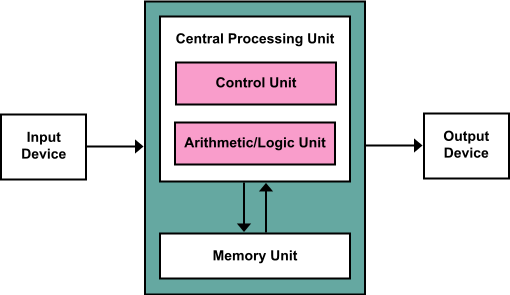
\includegraphics[height=0.65\textheight]{img/Von_Neumann_Architecture}\\[12pt]\Large
Stored-Program Computer Architecture (\cite{VonNeumann}, source: \href{http://en.wikipedia.org/wiki/Von_Neumann_architecture}{wikipedia})
\end{figure}
\end{frame}

\subsection{From Source To Instruction}
\begin{frame}[fragile]
\frametitle{\insertsectionhead{}: \insertsubsection{}}
\begin{block}{A simple app}
  \begin{pyglist}[language=c++,numbers=left,style=emacs]
  #include <iostream>

  int main(int argc, char *argv[])
  {
    int i = 42;
    std::cout << "i = " << i << "\n";
    return 0;
  }
  \end{pyglist}
\end{block}

\begin{block}{g++ simple_app.cpp -o simple_app}
  \begin{pyglist}[language=assembly,numbers=left,style=emacs]
    00000000004007e0 <main>:
    4007e0:	55                   	push   %rbp
    4007e1:	48 89 e5             	mov    %rsp,%rbp
    4007e4:	48 83 ec 20          	sub    $0x20,%rsp
    4007e8:	89 7d ec             	mov    %edi,-0x14(%rbp)
    4007eb:	48 89 75 e0          	mov    %rsi,-0x20(%rbp)
    4007ef:	c7 45 fc 2a 00 00 00 	movl   $0x2a,-0x4(%rbp)
    4007f6:	be 10 09 40 00       	mov    $0x400910,%esi
    4007fb:	bf 60 10 60 00       	mov    $0x601060,%edi
    400800:	e8 db fe ff ff       	callq  4006e0 <_ZStlsISt11char_traitsIcEERSt13basic_ostreamIcT_ES5_PKc@plt>
    400805:	8b 55 fc             	mov    -0x4(%rbp),%edx
    400808:	89 d6                	mov    %edx,%esi
    40080a:	48 89 c7             	mov    %rax,%rdi
    40080d:	e8 6e fe ff ff       	callq  400680 <_ZNSolsEi@plt>
    400812:	be 15 09 40 00       	mov    $0x400915,%esi
    400817:	48 89 c7             	mov    %rax,%rdi
    40081a:	e8 c1 fe ff ff       	callq  4006e0 <_ZStlsISt11char_traitsIcEERSt13basic_ostreamIcT_ES5_PKc@plt>
    40081f:	b8 00 00 00 00       	mov    $0x0,%eax
    400824:	c9                   	leaveq 
    400825:	c3                   	retq
  \end{pyglist}
  
\end{block}
\end{frame}

\begin{frame}
\frametitle{\insertsectionhead{}: \insertsubsection{}}
\begin{figure}[htb]
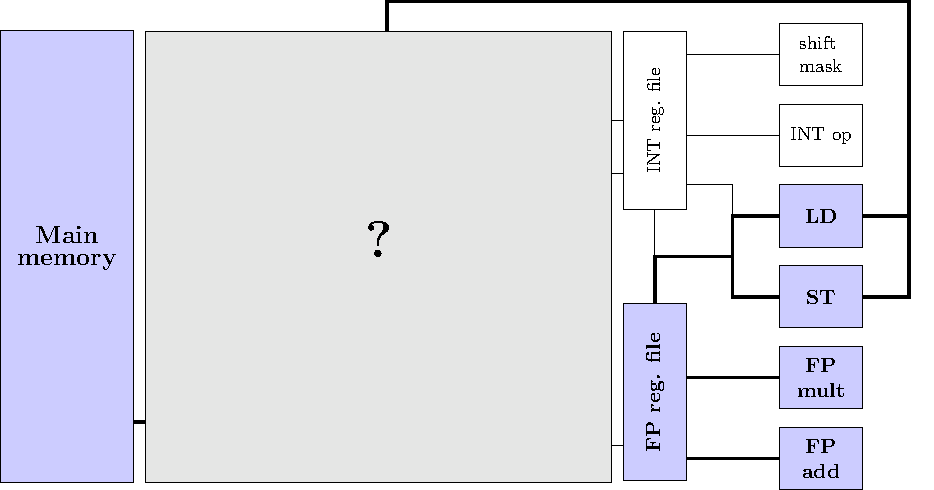
\includegraphics[height=0.65\textheight]{tikz/cachebased_microprocessor_matrix_memory_as_qm}\\[12pt]\Large
Block diagram Cache-based microprocessor (adapted from \cite{HagerWelleinIntroHPC}, Fig. 1.2)
\end{figure}
\end{frame}

\subsection{From Disk to Memory}
\begin{frame}
\frametitle{\insertsectionhead{}: \insertsubsection{}}
  
\begin{columns}[c]
  \begin{column}{.4\textwidth}
    \begin{figure}[htb]
      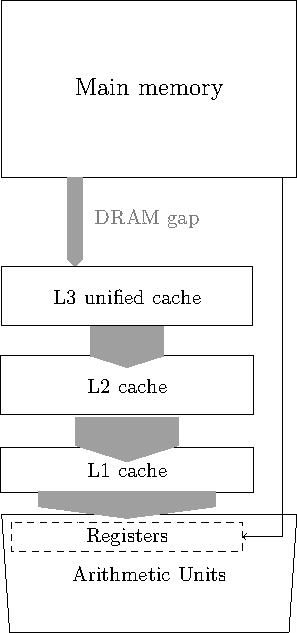
\includegraphics[height=0.65\textheight]{tikz/dram_gap}\\[12pt]\Large
      Memory hierarchy of a cache-based microprocessor (adapted from \cite{HagerWelleinIntroHPC}, Fig. 1.3)
    \end{figure}

  \end{column}
  \begin{column}{.57\textwidth}
    % laptop CPU, Intel(R) Core(TM) i7-3520M CPU @ 2.90GHz (Ivy Bridge)
    % $ getconf -a /usr|grep -i CACHE
    % LEVEL1_ICACHE_SIZE                 32768
    % LEVEL1_ICACHE_ASSOC                8
    % LEVEL1_ICACHE_LINESIZE             64
    % LEVEL1_DCACHE_SIZE                 32768
    % LEVEL1_DCACHE_ASSOC                8
    % LEVEL1_DCACHE_LINESIZE             64
    % LEVEL2_CACHE_SIZE                  262144
    % LEVEL2_CACHE_ASSOC                 8
    % LEVEL2_CACHE_LINESIZE              64
    % LEVEL3_CACHE_SIZE                  4194304
    % LEVEL3_CACHE_ASSOC                 16
    % LEVEL3_CACHE_LINESIZE              64
    % server grade CPU, Intel(R) Xeon(R) CPU E5-2630 0 @ 2.30GHz (Sandy Bridge)
    % $ getconf -a /usr|grep -i CACHE
    % LEVEL1_ICACHE_SIZE                 32768
    % LEVEL1_ICACHE_ASSOC                8
    % LEVEL1_ICACHE_LINESIZE             64
    % LEVEL1_DCACHE_SIZE                 32768
    % LEVEL1_DCACHE_ASSOC                8
    % LEVEL1_DCACHE_LINESIZE             64
    % LEVEL2_CACHE_SIZE                  262144
    % LEVEL2_CACHE_ASSOC                 8
    % LEVEL2_CACHE_LINESIZE              64
    % LEVEL3_CACHE_SIZE                  15728640
    % LEVEL3_CACHE_ASSOC                 20
    % LEVEL3_CACHE_LINESIZE              64
    % server grade CPU, Intel(R) Xeon(R) CPU E5-2640 0 @ 2.50GHz (Sandy Bridge)
    % $ getconf -a /usr|grep -i CACHE
    % LEVEL1_ICACHE_SIZE                 32768
    % LEVEL1_ICACHE_ASSOC                8
    % LEVEL1_ICACHE_LINESIZE             64
    % LEVEL1_DCACHE_SIZE                 32768
    % LEVEL1_DCACHE_ASSOC                8
    % LEVEL1_DCACHE_LINESIZE             64
    % LEVEL2_CACHE_SIZE                  262144
    % LEVEL2_CACHE_ASSOC                 8
    % LEVEL2_CACHE_LINESIZE              64
    % LEVEL3_CACHE_SIZE                  15728640
    % LEVEL3_CACHE_ASSOC                 20
    % LEVEL3_CACHE_LINESIZE              64
    % server grade CPU, Intel(R) Xeon(R) CPU E3-1245 v3 @ 3.40GHz
    % $ getconf -a /usr|grep -i CACHE
    % LEVEL1_ICACHE_SIZE                 32768
    % LEVEL1_ICACHE_ASSOC                8
    % LEVEL1_ICACHE_LINESIZE             64
    % LEVEL1_DCACHE_SIZE                 32768
    % LEVEL1_DCACHE_ASSOC                8
    % LEVEL1_DCACHE_LINESIZE             64
    % LEVEL2_CACHE_SIZE                  262144
    % LEVEL2_CACHE_ASSOC                 8
    % LEVEL2_CACHE_LINESIZE              64
    % LEVEL3_CACHE_SIZE                  8388608
    % LEVEL3_CACHE_ASSOC                 16
    % LEVEL3_CACHE_LINESIZE              64
    \begin{description}
    \item[L3 unified cache] $\unit[4-15]{MB}$ 
    \item[L2 cache] $N_{c}\times\unit[256]{KB}$ 
    \item[L1 cache] $N_{c}\times2\times\unit[32]{KB}$ 
    \item[cache line size] $\unit[64]{B} = \unit[8]{float32} = \unit[4]{double}$ 
    \end{description}
  \end{column}
\end{columns}
\end{frame}

\begin{frame}
\frametitle{\insertsectionhead{}: \insertsubsection{}}
  
    \begin{figure}[htb]
      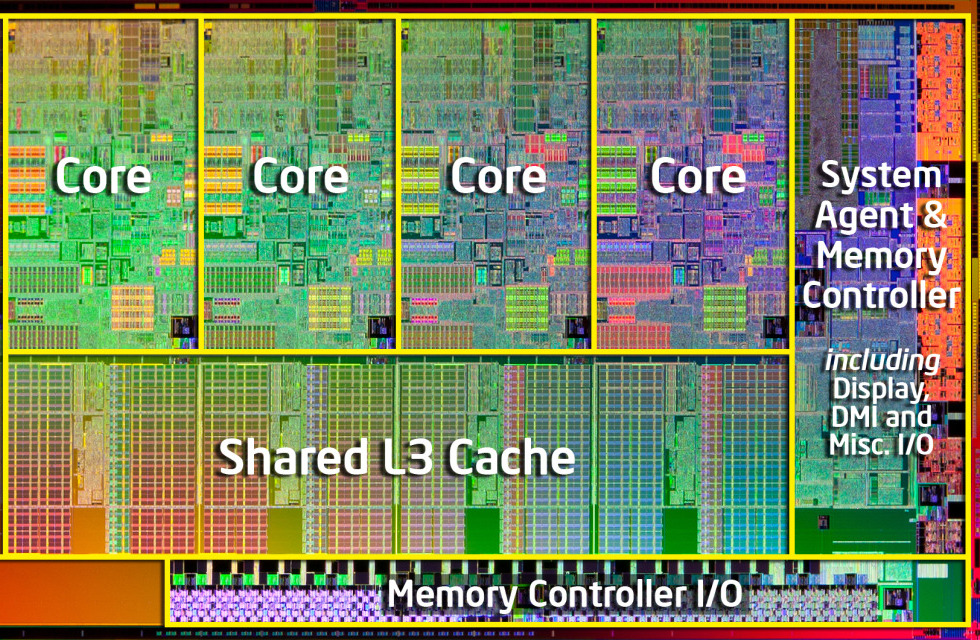
\includegraphics[height=0.65\textheight]{img/sandy-bridge-die-map_noIGP}\\[12pt]\Large
      Intel\textregistered{} Sandy Bridge \textregistered{} Die Map (\href{http://www.bit-tech.net/hardware/cpus/2011/01/03/intel-sandy-bridge-review/1}{bit-tech.net})
    \end{figure}

    \begin{itemize}
    \item memory/data related  
    \end{itemize}
\end{frame}


\subsection{Exploring it all}
\begin{frame}
\frametitle{\insertsectionhead{}: \insertsubsection{}}
\end{frame}

\section[Measurement]{The time needed}
\subsection{\texttt{time}}
\begin{frame}
\frametitle{\insertsectionhead{}: \insertsubsectionhead{}}
\end{frame}

\subsection{\texttt{perf}}
\begin{frame}
\frametitle{\insertsectionhead{}: \insertsubsectionhead{}}
\end{frame}

\subsection{\texttt{valgrind}}
\begin{frame}
\frametitle{\insertsectionhead{}: \insertsubsectionhead{}}
\end{frame}


\part{Tour de Force}
\section{The Blessings of Design}
\subsection{Inheritance}
\begin{frame}
\frametitle{\insertsectionhead{}: \insertsubsectionhead{}}
\end{frame}

\subsection{Over-Objectivism}
\begin{frame}
\frametitle{\insertsectionhead{}: \insertsubsectionhead{}}
\end{frame}

\subsection{Take-Home}
\begin{frame}
\frametitle{\insertsectionhead{}: \insertsubsectionhead{}}
\end{frame}

\section{The Free Lunch}
\section{Real-Life HPC}


\part{Exercises}
\section{Tasks}
\section{Results}

\section{Literature}
\begin{frame}[c]
\frametitle{\insertsection{}}
\nocite{*}
\tiny%footnotesize
\bibliographystyle{ieeetr}
\bibliography{slides}
\end{frame}

\end{document}




